\documentclass[a4paper]{article}
\usepackage[utf8]{vntex}
\usepackage[english]{babel}
\usepackage[utf8]{inputenc}
\usepackage{amsmath,graphicx,xcolor,booktabs,array,indentfirst}
\usepackage[margin=25mm,headheight=32pt,headsep=8mm]{geometry}
\usepackage{fancyhdr,listings}
\usepackage[colorlinks=true,linkcolor=black,citecolor=black,urlcolor=blue]{hyperref}
\setlength{\parindent}{1cm}
\setlength{\parskip}{0pt}
\setlength{\emergencystretch}{2em}
\raggedbottom
\clubpenalty=10000
\widowpenalty=10000
\pagestyle{fancy}
\fancyhf{}
\fancyhead[R]{%
\begin{tabular}{@{}r@{\hspace{2mm}}c@{}}
\begin{tabular}{@{}r@{}}
\small Ho Chi Minh City University of Technology\\
\small Faculty of Computer Science and Engineering
\end{tabular}&\raisebox{-2mm}{
\includegraphics[width=8mm]{hcmut_logo.png}}
\end{tabular}}
\fancyfoot[L]{\footnotesize Microprocessors--Microcontrollers Laboratory (CO3010)}
\fancyfoot[R]{\footnotesize\thepage}
\renewcommand{\headrulewidth}{0.3pt}
\definecolor{codeblue}{RGB}{0,83,160}
\definecolor{codebg}{RGB}{247,248,250}
\lstset{language=C,basicstyle=\ttfamily\small,
keywordstyle=\color{codeblue}\bfseries,stringstyle=\color{red!60!black},
numbers=left,numberstyle=\tiny\color{gray},numbersep=7pt,
frame=single,rulecolor=\color{gray!40},backgroundcolor=\color{codebg},
breaklines=true,breakatwhitespace=false,keepspaces=true,
columns=fullflexible,tabsize=4,showstringspaces=false,
captionpos=t,aboveskip=10pt,belowskip=10pt,xleftmargin=12pt,
framexleftmargin=3pt}
\newcommand{\code}[1]{\texttt{\detokenize{#1}}}
\newcommand{\topic}[1]{\subsection{#1}}
\begin{document}
\hypersetup{pageanchor=false}
\begin{titlepage}
\centering
{\large VIETNAM NATIONAL UNIVERSITY HO CHI MINH CITY\par}
\vspace{3mm}
{\large HO CHI MINH CITY UNIVERSITY OF TECHNOLOGY\par}
\vspace{3mm}
{\large FACULTY OF COMPUTER SCIENCE AND ENGINEERING\par}
\vspace{15mm}

\includegraphics[width=4cm]{hcmut_logo.png}\par
\vspace{13mm}
\par{\Large\bfseries Microprocessors--Microcontrollers Laboratory\par}
{\Large\bfseries (CO3010)\par}
\vspace{8mm}
\rule{\textwidth}{0.5pt}\par
\vspace{6mm}
{\Large\bfseries Laboratory Report\par}
\vspace{6mm}
{\LARGE\bfseries LAB 05\par}
\vspace{4mm}
{\Large\bfseries UART Communication and ADC Data Transfer\par}
\vspace{6mm}
\rule{\textwidth}{0.5pt}\par
\vspace{18mm}
\begin{tabular}{rl}
Advisor: & Phan Văn Sỹ\\[3mm]
Student: & Nguyễn Cáp Quốc Khánh\\[3mm]
Student ID: & 2452500\\[3mm]
Class: & CC03
\end{tabular}
\vfill
{\small HO CHI MINH CITY, NOVEMBER 2026\par}
\end{titlepage}
\hypersetup{pageanchor=true}
\pagenumbering{roman}
\begingroup
\small
\setcounter{tocdepth}{1}
\tableofcontents
\endgroup
\clearpage
\listoffigures
\listoftables
\clearpage
\pagenumbering{arabic}

\section*{Overview}
\addcontentsline{toc}{section}{Overview}
This laboratory develops a request--response link between an STM32
microcontroller and a serial terminal. The terminal requests an analog sample
using \texttt{!RST\#}; the controller reads ADC1 and returns an ASCII frame such as
\texttt{!ADC=2048\#}. Acknowledgment with \texttt{!OK\#} completes the exchange.
If acknowledgment does not arrive, the controller retransmits the saved
response after a three-second waiting interval. The same measurement remains
associated with the transaction until it is acknowledged.

Two finite state machines divide the problem into manageable parts. A command
parser recognizes complete frames in a stream of received bytes. A communication
controller decides when to acquire a sample, transmit it, wait, retry, and return
to the idle state. A ring buffer connects interrupt-driven reception to these
foreground tasks. A separate LED heartbeat demonstrates how periodic work can
continue while the application waits for commands or acknowledgment.

The implementation follows the protocol and module structure of the laboratory
handout\cite{lab}. Its peripheral settings and code excerpts describe the supplied
project. STM32 documentation supports the ADC and HAL explanations\cite{stm32,hal};
Keil and Proteus provide the development and simulation context\cite{keil,proteus}.
The discussion connects each design decision to the resulting behavior, including
frame recovery, timeout calculation, saved-packet retransmission, and the visible
midscale ADC result.


\section{Communication principles and laboratory objectives}

\topic{Why a protocol is required above UART}

UART transfers individual characters, but a complete application must also
identify the beginning and end of a command, decide which commands are valid,
and know whether a response has been accepted. These responsibilities belong
to the application protocol. Correct baud-rate and pin settings establish the
byte channel; framing and acknowledgment establish the meaning of those bytes.

The protocol uses \code{!} as a start delimiter and \texttt{\#} as an end delimiter.
The payload between them is case-sensitive. Therefore, \texttt{!RST\#} and
\texttt{!OK\#} are valid commands, while \texttt{!rst\#} is not. A received byte does
not immediately become a command: the parser must first collect and validate
the entire delimited payload. This distinction prevents a partial or unrelated
character sequence from accidentally starting an ADC conversion.

Flow control regulates how much unacknowledged information is outstanding.
Here, only one response transaction is active at a time. The controller sends
one sample and waits for acknowledgment before accepting another request as
a new measurement. Error recovery is provided by a timeout and retransmission.
This is a simple stop-and-wait acknowledgment scheme. It does not include a
checksum, sequence number, or negative acknowledgment, so retransmission alone
does not provide complete detection of arbitrary data corruption.


\topic{Required behavior and implementation decisions}

\begin{table}[htbp]\centering\small
\caption{Protocol messages and their interpretation}
\begin{tabular}{p{25mm}p{38mm}p{83mm}}\toprule
Message & Direction & Meaning\\\midrule
\texttt{!RST\#} & Terminal to STM32 & Request one new sample while idle.\\
\texttt{!ADC=n\#} & STM32 to terminal & Return the saved decimal ADC value.\\
\texttt{!OK\#} & Terminal to STM32 & Acknowledge the outstanding response.\\
No acknowledgment & Internal timeout & Send the same saved packet again after 3000 ms.\\\bottomrule
\end{tabular}\end{table}

The core acceptance conditions are a recognizable request, one valid ADC
measurement, correctly formatted output, repeated transmission of the same
value on timeout, and completion on acknowledgment. The final firmware adds
bounded receive buffering and diagnostic counters to these basic requirements.
It also defines behavior for unexpected commands: OK is ignored while idle,
and RST is ignored while waiting for acknowledgment. The latter rule preserves
the identity of the outstanding measurement.

The handout progresses through circuit setup, peripheral configuration,
loop-back, sensor reading, command parsing, and integration of two FSMs.
These stages are discussed in that order before the final simulation results.
The final project contains the integrated protocol rather than an always-on
echo program or an unconditional stream of ADC samples.


\section{Proteus platform and signal connections}

\topic{Circuit structure}

Figure~\ref{fig:schematic} shows the supplied circuit before the terminal
transaction is displayed. The potentiometer generates a variable analog
voltage between ground and 3.3 V. Its wiper drives the non-inverting input
of the operational amplifier. Negative feedback connects the amplifier output
to its inverting input through R1. With ideal input current, almost no voltage
is dropped across R1; the output follows the wiper voltage. This is a voltage
follower, rather than a gain stage with a gain of ten.

The follower presents a high input impedance to the potentiometer and a low
output impedance to the ADC input. Its output is connected to PA0 through the
\code{ADC0} net. The voltmeter displays the analog level applied to the follower
input. In the running result, the voltage is approximately 1.65 V, halfway
between the supply rails. The first circuit image is used to explain wiring;
its inactive meter indication is not treated as an ADC measurement.

\begin{figure}[htbp]\centering
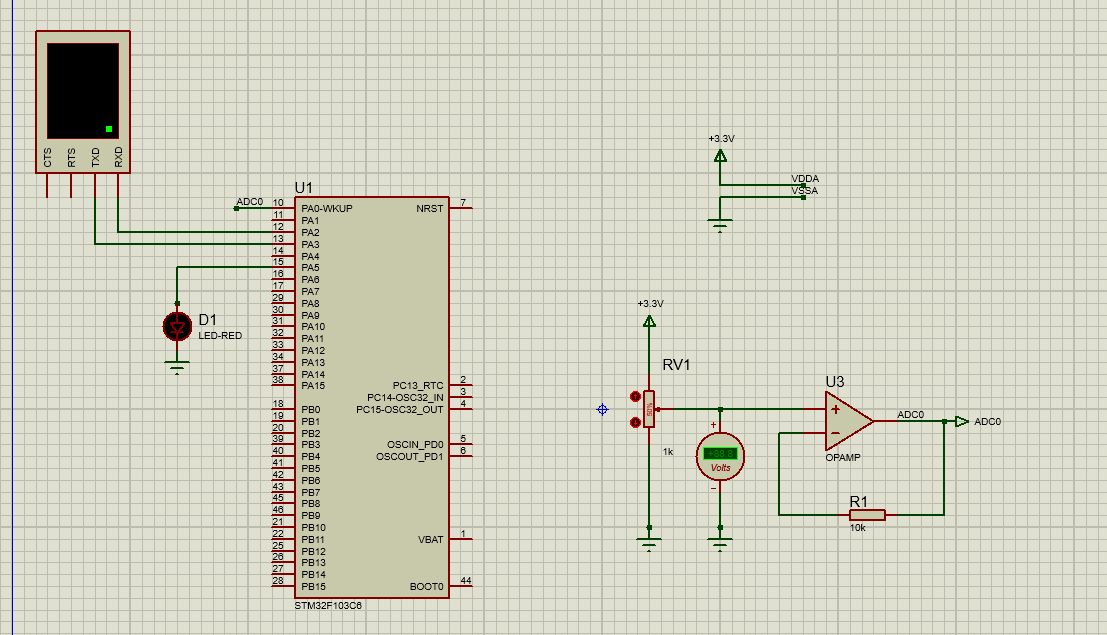
\includegraphics[width=\textwidth]{lab5_schematic.png}
\caption{Proteus circuit with USART2, a variable analog input, and a voltage follower.}
\label{fig:schematic}\end{figure}


\topic{Pin allocation and terminal wiring}

\begin{table}[htbp]\centering
\caption{Signal allocation in the supplied project}
\begin{tabular}{lll}\toprule
Pin & Peripheral or mode & Application role\\\midrule
PA0 & ADC1 channel 0, analog & Buffered potentiometer voltage\\
PA2 & USART2 TX, alternate-function output & Transmit ADC packets\\
PA3 & USART2 RX, input & Receive terminal commands\\
PA5 & Push-pull GPIO output & Red heartbeat LED\\\bottomrule
\end{tabular}\end{table}

The terminal RXD pin receives the microcontroller TX signal from PA2.
The terminal TXD pin drives the microcontroller RX input on PA3. Thus, TX and
RX are crossed between endpoints. Both endpoints use a common ground and the
same serial parameters. The RTS and CTS pins are unused because hardware flow
control is disabled. Application acknowledgment is implemented by the OK frame,
not by an RTS/CTS handshake.

The LED on PA5 is active high in the circuit. It starts low and is toggled
every 500 ms by the foreground application. The blink period is 1000 ms,
because an ON interval and an OFF interval are both needed for one complete
cycle. This LED is independent of the ADC packet: it is a heartbeat, not an
acknowledgment indicator.


\section{Project configuration and timing calculations}

\topic{System clock, USART2, and interrupt configuration}

The system clock uses the internal 8-MHz HSI oscillator with no PLL.
AHB, APB1, and APB2 are undivided. Consequently, USART2 receives an 8-MHz
peripheral clock from APB1. Its configured baud rate is 9600 bits/s with eight
data bits, no parity, one stop bit, and 16-times oversampling. Both transmission
and reception are enabled. The terminal must use the same 9600/8-N-1 format.


\par\noindent\begin{minipage}{\linewidth}
\begin{lstlisting}[caption={Essential USART2 parameters},firstnumber=1]
huart2.Instance = USART2;
huart2.Init.BaudRate = 9600;
huart2.Init.WordLength = UART_WORDLENGTH_8B;
huart2.Init.StopBits = UART_STOPBITS_1;
huart2.Init.Parity = UART_PARITY_NONE;
huart2.Init.Mode = UART_MODE_TX_RX;
huart2.Init.HwFlowCtl = UART_HWCONTROL_NONE;
huart2.Init.OverSampling = UART_OVERSAMPLING_16;
\end{lstlisting}
\end{minipage}\par

An 8-N-1 character occupies ten transmitted bits: one start bit, eight data
bits, and one stop bit. Therefore,
\[
T_{\mathrm{bit}}=\frac{1}{9600}\approx104.17\ \mu\mathrm{s},\qquad
T_{\mathrm{char}}=\frac{10}{9600}\approx1.042\ \mathrm{ms}.
\]
The five-character request \texttt{!RST\#} takes approximately 5.21 ms on the wire,
while the four-character acknowledgment \texttt{!OK\#} takes about 4.17 ms.
These values describe serial transfer time; parser service and foreground
execution add their own latency.

The USART2 global interrupt is enabled with preemption priority zero. Its
handler calls \code{HAL_UART_IRQHandler(&huart2)}, allowing the HAL driver to
complete the active receive operation and invoke the receive callback.
SysTick has a lower interrupt priority and supplies the default millisecond
HAL time base. Short receive callbacks help prevent the UART interrupt from
unnecessarily delaying other processing.


\topic{ADC1 configuration and conversion time}

ADC1 uses channel 0 on PA0, right-aligned data, one regular conversion,
software triggering, and disabled scan, continuous, and discontinuous modes.
Each accepted request explicitly starts one conversion. Merely reading the ADC
data register is insufficient to guarantee a new measurement in this mode.


\par\noindent\begin{minipage}{\linewidth}
\begin{lstlisting}[caption={Essential ADC1 parameters},firstnumber=1]
hadc1.Instance = ADC1;
hadc1.Init.ScanConvMode = ADC_SCAN_DISABLE;
hadc1.Init.ContinuousConvMode = DISABLE;
hadc1.Init.DiscontinuousConvMode = DISABLE;
hadc1.Init.ExternalTrigConv = ADC_SOFTWARE_START;
hadc1.Init.DataAlign = ADC_DATAALIGN_RIGHT;
hadc1.Init.NbrOfConversion = 1;
sConfig.Channel = ADC_CHANNEL_0;
sConfig.Rank = ADC_REGULAR_RANK_1;
sConfig.SamplingTime = ADC_SAMPLETIME_55CYCLES_5;
\end{lstlisting}
\end{minipage}\par

APB2 is divided by two for the ADC clock, giving
\(f_{\mathrm{ADC}}=8/2=4\) MHz. The selected acquisition interval is 55.5 ADC
clock cycles. Adding the 12.5-cycle conversion interval gives the nominal
sampling-plus-conversion duration\cite{stm32}:
\[
T_{\mathrm{ADC}}=\frac{55.5+12.5}{4\times10^6}
=17\ \mu\mathrm{s}.
\]
This calculation excludes software-call and trigger overhead. The 10-ms
polling timeout in the sensor driver is an upper waiting limit for a conversion
to finish; it does not mean that one sample is intentionally taken every 10 ms.
The nominal ADC conversion is much shorter than a single UART response.


\topic{Millisecond time base and LED service}

The project does not use a separate TIM2 software-timer module for its
three-second timeout. \code{HAL_Init} establishes the HAL time base, and
\code{SysTick_Handler} calls \code{HAL_IncTick}. The application compares
\code{HAL_GetTick()} with saved timestamps. Waiting is expressed as a condition
tested on each foreground pass, rather than a three-second blocking delay.

The same elapsed-time pattern services the LED. Since the main loop remains
available during the acknowledgment wait, reception, parsing, and heartbeat
updates can continue. ADC polling and UART transmission are still bounded
blocking operations; the complete application is therefore cooperative, not
fully asynchronous in every peripheral operation.


\section{Preliminary UART loop-back}

\topic{Purpose and expected observation}

Loop-back is the first functional check of the serial channel. A character
typed at the terminal is received by the STM32 and transmitted back unchanged.
For example, sending \texttt{A7\#} should produce the same three characters in
the same order. A successful test supports the TX/RX wiring, terminal baud-rate
agreement, interrupt path, and ability to transmit from the firmware.

The handout illustrates an echo directly inside the receive callback. In the
integrated project, the callback instead stores bytes in a ring buffer, and
the foreground decides what to do with them. The following isolated test loop
uses that receive driver to echo bytes outside the interrupt. It is a temporary
alternative to the parser and communication calls, not an additional loop
to run alongside them. The receive driver must already have been initialized.


\par\noindent\begin{minipage}{\linewidth}
\begin{lstlisting}[caption={Optional foreground loop-back test},firstnumber=1]
while (1)
{
    uint8_t test_byte;
    UART_RxService();
    if (UART_RxPop(&test_byte))
    {
        HAL_UART_Transmit(&huart2, &test_byte, 1, 50);
    }
}
\end{lstlisting}
\end{minipage}\par

Both the loop-back test and the protocol parser consume the same receive
queue. Running them together would let one consumer remove bytes needed by
the other. Only one of these foreground modes should own the byte stream.
For verification, terminal local echo should be disabled or clearly identified;
otherwise, seeing the typed characters alone would not prove that the STM32
returned them.

The supplied final-protocol image is not a separate loop-back capture. Its
visible request text can be produced by terminal local echo, because the final
receive callback does not transmit each incoming byte. A dedicated echo test
would document this preliminary stage independently.


\section{Sensor acquisition and ADC interpretation}

\topic{Twelve-bit conversion and the midscale value}

The STM32F103 ADC resolution is 12 bits\cite{stm32}. It provides
\(2^{12}=4096\) possible output codes, numbered 0 through 4095. Thus, 4096
is the number of levels, not a valid 12-bit output code. For this 3.3-V circuit,
the ideal quantization step is
\[
q=\frac{V_{\mathrm{REF}}}{4096}
=\frac{3.3}{4096}\approx0.8057\ \mathrm{mV}.
\]
Away from the upper saturation limit, an idealized code model is
\[
D\approx\left\lfloor\frac{V_{\mathrm{in}}}{V_{\mathrm{REF}}}\,4096\right\rfloor,
\qquad 0\leq D\leq4095.
\]
For \(V_{\mathrm{in}}=1.65\) V and \(V_{\mathrm{REF}}=3.3\) V,
\[
D\approx\frac{1.65}{3.3}\,4096=2048.
\]
The running screenshot therefore has the expected midscale relationship:
the voltmeter displays approximately 1.65 V and the response contains 2048.
Quantization, reference-voltage variation, and ADC error can affect a real
measurement, so the ideal equation describes the expected relationship rather
than a calibration certificate. The handout's description of a 13-bit ADC and
a 5-V full scale is not the configuration of this STM32 circuit.


\topic{Starting, waiting for, reading, and stopping a conversion}

\par\noindent\begin{minipage}{\linewidth}
\begin{lstlisting}[caption={One valid sample per accepted request},firstnumber=1]
HAL_StatusTypeDef Sensor_ReadOnce(uint32_t *value){

    HAL_StatusTypeDef status = HAL_ADC_Start(&hadc1);
    if(status != HAL_OK) return status;

    status = HAL_ADC_PollForConversion(&hadc1, 10);
    if(status == HAL_OK){

        *value = HAL_ADC_GetValue(&hadc1);
    }

    (void)HAL_ADC_Stop(&hadc1);
    return status;
}
\end{lstlisting}
\end{minipage}\par

The output parameter points to the caller's sample variable.
\code{HAL_ADC_Start} enables the requested software conversion.
\code{HAL_ADC_PollForConversion} waits until conversion completes or the timeout
expires. The driver writes the caller's variable only after successful
completion, then stops the ADC even if polling failed. Returning the status
lets the communication FSM distinguish a valid sample from an acquisition error.

A numerical zero is a legitimate result when the input is near ground.
Consequently, the program does not use zero as a substitute for an ADC error.
If acquisition fails, it increments \code{adc_read_errors}, stays idle, and
sends no fabricated measurement. The terminal can issue another request after
the cause has been resolved.


\topic{Calibration and the simulation-specific branch}

Startup calls \code{Sensor_Init} before enabling command reception. This
function first attempts the standard HAL ADC calibration routine. The supplied
project explicitly enables a Proteus compatibility option. If the standard
routine fails while the reset-calibration bit remains set, the compatibility
branch clears that bit, starts calibration, and still waits for the calibration
bit to clear. It has a 20-ms timeout and returns failure if completion does not
occur. The application enters its error handler if sensor initialization fails.

This branch is a conditional accommodation in the supplied simulation code,
not a general replacement for hardware calibration. For a physical board,
the compatibility argument is intended to be zero. The protocol and ADC
conversion explanation do not depend on displaying low-level register code;
the essential application contract is successful sensor initialization followed
by a checked conversion for each newly accepted request.


\section{Interrupt reception and the receive buffer}

\topic{Module responsibilities and data movement}

Figure~\ref{fig:dataflow} summarizes the division of work. The UART interrupt
captures a single byte and quickly enables the next receive operation. The
main loop removes queued bytes and recognizes commands. The communication FSM
then acts on those commands. ADC conversion and packet transmission occur in
the foreground, keeping substantial work out of the receive interrupt.

\begin{figure}[htbp]\centering
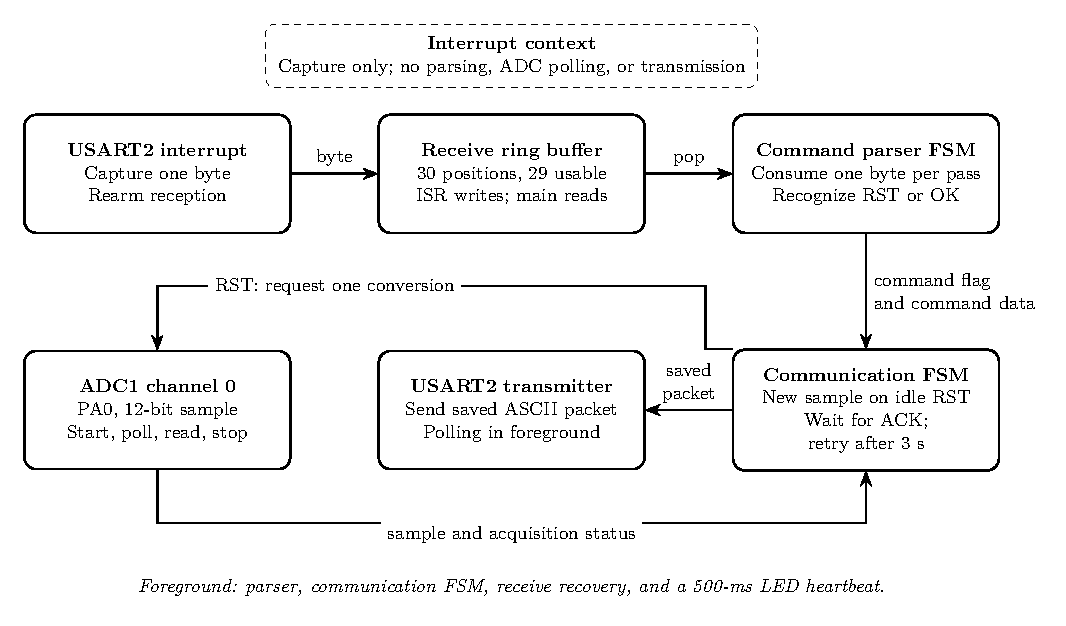
\includegraphics[width=\textwidth]{lab5_dataflow.pdf}
\caption{Data flow from interrupt reception to a saved ADC response.}
\label{fig:dataflow}\end{figure}

Reception, command recognition, transaction control, and ADC access are
implemented in separate source modules.
The receive module hides the buffer indices behind functions for initialization,
service, pop, and flush. The parser exports a command mailbox rather than its
partially collected token. This keeps an incomplete frame from reaching the
communication controller.


\topic{Why a 30-slot ring buffer stores at most 29 bytes}

The receive array contains 30 byte positions. The write index identifies
the next insertion position, while the read index identifies the oldest unread
byte. Equal indices mean empty. Before insertion, the producer calculates
\[
w_{\mathrm{next}}=(w+1)\bmod30.
\]
If this next position equals the read index, insertion would make the full
buffer indistinguishable from an empty buffer. One position is therefore left
unused, giving 29 usable bytes. For example, incrementing an index from 29
wraps it to zero. The consumer applies the same wrap rule when removing data.

The interrupt publishes the new write index only after storing the byte.
The foreground advances the read index only after copying the old byte to
the caller. Each side normally modifies its own index, giving a single-producer,
single-consumer arrangement. Shared interrupt state is declared appropriately
in the driver; command variables exchanged only between the two foreground
FSM calls do not need that same interrupt-sharing treatment.


\par\noindent\begin{minipage}{\linewidth}
\begin{lstlisting}[caption={Receive completion: enqueue one byte and enable the next receive},firstnumber=1]
void HAL_UART_RxCpltCallback(UART_HandleTypeDef *huart)
{
    if (huart->Instance != USART2) return;

    uint8_t next = (uint8_t)((rx_write + 1u) % RX_SIZE);
    if (next == rx_read) {
        uart_rx_dropped++;
    } else {
        rx_buffer[rx_write] = rx_byte;
        rx_write = next;
    }
    RxArm();
}
\end{lstlisting}
\end{minipage}\par

\par\noindent\begin{minipage}{\linewidth}
\begin{lstlisting}[caption={Remove the oldest unread byte without waiting},firstnumber=1]
uint8_t UART_RxPop(uint8_t *byte)
{
    if (rx_read == rx_write) return 0;
    *byte = rx_buffer[rx_read];
    rx_read = (uint8_t)((rx_read + 1u) % RX_SIZE);
    return 1;
}
\end{lstlisting}
\end{minipage}\par

\topic{Rearming reception and recovering after data loss}

\code{HAL_UART_Receive_IT} is armed for one byte, not an entire command.
After that byte arrives, completion of the operation does not by itself create
a new application receive request. The callback calls \code{RxArm} again.
Initialization arms the first receive once; the main loop does not repeatedly
restart a successful active receive operation.

If rearming fails, the driver increments \code{uart_rx_errors} and sets a
pending service flag. \code{UART_RxService} attempts the rearm from the main
loop. The UART error callback also records an error and requests service.
Neither error path invents a received byte.

When the queue is full, the new byte is dropped and
\code{uart_rx_dropped} increases. The parser watches both diagnostic counters.
Any change invalidates the frame under construction: the parser returns to
its waiting state, clears its token length, and flushes old queued bytes. The
flush protects its index update with a brief interrupt-state-preserving critical
section. This recovery intentionally discards uncertain data rather than
combining fragments across a known loss. A subsequent complete frame beginning
with a fresh start delimiter can be recognized normally.


\section{Command parser finite state machine}

\topic{States, transitions, and framing rules}

The parser has two states. \code{WAIT_START} ignores bytes until a start
delimiter is received. \code{COLLECT} appends payload characters until the end
delimiter arrives or the token becomes too long. The token array has four
positions: three payload characters for RST and one null terminator required
by C string comparison. OK uses only two payload characters.

\begin{figure}[htbp]\centering
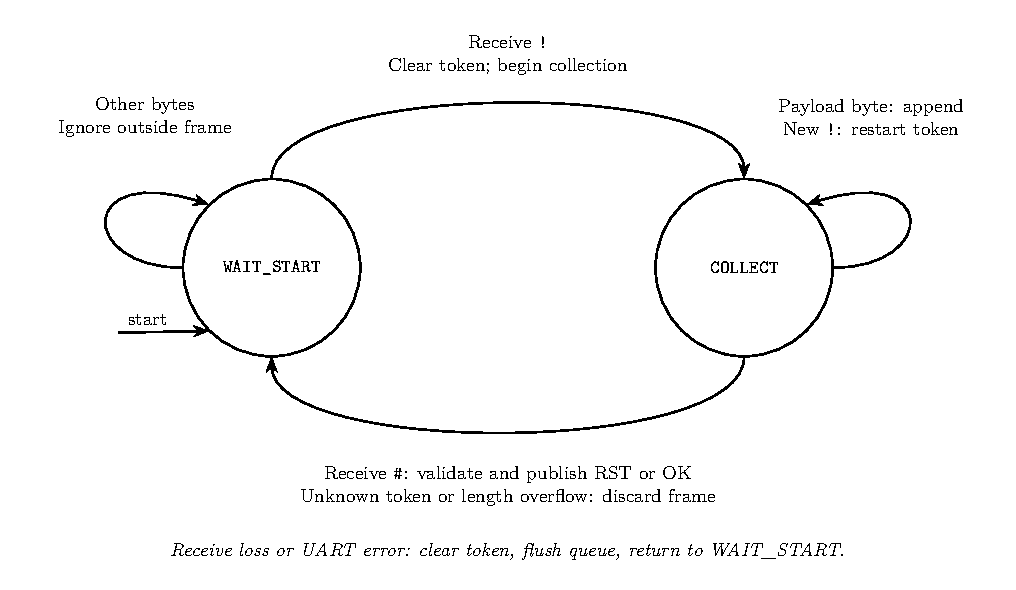
\includegraphics[width=\textwidth]{lab5_parser_fsm.pdf}
\caption{Two-state parser with delimiter resynchronization and bounded token storage.}
\label{fig:parser}\end{figure}

A start delimiter is handled before the state-specific checks. Receiving a
new \code{!} therefore starts a new candidate token even when a previous frame
was unfinished. An end delimiter terminates the C string and triggers exact
comparison with RST and OK. A matching token produces a command; an unknown
token produces no command. Either way, processing the end delimiter returns
the parser to \code{WAIT_START}.


\topic{Recognizing one byte at a time}

\par\noindent\begin{minipage}{\linewidth}
\begin{lstlisting}[caption={Command parser and publication of a complete command},firstnumber=1]
void command_parser_fsm(void)
{
    uint8_t byte;

    if (seen_dropped != uart_rx_dropped || seen_errors != uart_rx_errors) {
        seen_dropped = uart_rx_dropped;
        seen_errors = uart_rx_errors;
        state = WAIT_START;
        length = 0;
        UART_RxFlush();
    }

    if (command_flag || !UART_RxPop(&byte)) return;

    if (byte == '!') {
        state = COLLECT;
        length = 0;
        return;
    }
    if (state != COLLECT) return;

    if (byte == '#') {
        token[length] = '\0';
\end{lstlisting}
\end{minipage}\par

\par\noindent\begin{minipage}{\linewidth}
\begin{lstlisting}[caption={Command parser and publication of a complete command (continued)},firstnumber=24]
        if (strcmp(token, "RST") == 0) {
            command_data = CMD_RST;
            command_flag = 1;
        } else if (strcmp(token, "OK") == 0) {
            command_data = CMD_OK;
            command_flag = 1;
        }
        state = WAIT_START;
        length = 0;
        return;
    }

    if (length < sizeof(token) - 1u) {
        token[length++] = (char)byte;
    } else {
        state = WAIT_START;
        length = 0;
    }
}
\end{lstlisting}
\end{minipage}\par

At most one byte is removed during each call. This bounds the foreground
work per parser pass and lets the communication controller check its timeout
and the LED update frequently. A complete RST request needs five such parser
passes after the bytes become available. These passes normally occur much
faster than the human typing rate; they are not separated by a fixed delay.

The statement \code{token[length] = '\0'} creates a valid C string before
\code{strcmp}. Since the payload length never exceeds three, this write remains
inside the four-position array. \code{strcmp} returns zero when strings are
equal, which is why the comparisons explicitly test \code{== 0}. Prefixes
alone do not match: a partial R or RS is not RST.

The output mailbox consists of \code{command_data} and \code{command_flag}.
The parser writes the command kind and then raises the flag. While a command
is pending, it does not pop another byte. The communication FSM consumes and
clears the mailbox later in the same main-loop pass. Thus, a newly parsed
command cannot be overwritten by a second one before the controller sees it;
later bytes remain queued in arrival order.


\topic{Examples of valid input and recovery}

\begin{table}[htbp]\centering\small
\caption{Parser behavior for representative input streams}
\begin{tabular}{p{40mm}p{106mm}}\toprule
Input stream & Result\\\midrule
\texttt{!RST\#} & Publish CMD\_RST after the final delimiter.\\
\texttt{!OK\#} & Publish CMD\_OK after the final delimiter.\\
\texttt{abc!RST\#} & Ignore leading characters, then recognize RST.\\
\code{!RS} & Remain in COLLECT; no complete command yet.\\
\texttt{!RS!OK\#} & Restart at the second start delimiter and recognize OK.\\
\texttt{!rst\#} or \texttt{!\#} & Reject the unknown or empty token.\\
\texttt{!RSTX\#} & Discard the oversized token; wait for another start delimiter.\\
\texttt{!OK\#\textbackslash{}r\textbackslash{}n} & Recognize OK; ignore CR/LF outside the frame.\\\bottomrule
\end{tabular}\end{table}

These examples describe the inspected algorithm rather than additional
terminal measurements. They show how delimiter recognition, length checking,
and exact token matching work together. There is no parser timeout for an
unfinished frame; a later start delimiter can resynchronize it. Because the
parser bounds storage independently of input length, a long malformed token
does not require an equally large token array.


\section{Communication finite state machine}

\topic{Idle and acknowledgment-wait states}

The communication controller has two states. In \code{COMM_IDLE}, a valid
RST starts a new transaction: acquire one sample, construct the response,
save its length, enter \code{COMM_WAIT_ACK}, and attempt transmission.
In \code{COMM_WAIT_ACK}, OK completes the transaction; otherwise, elapsed
time determines whether the saved packet must be resent.

\begin{figure}[htbp]\centering
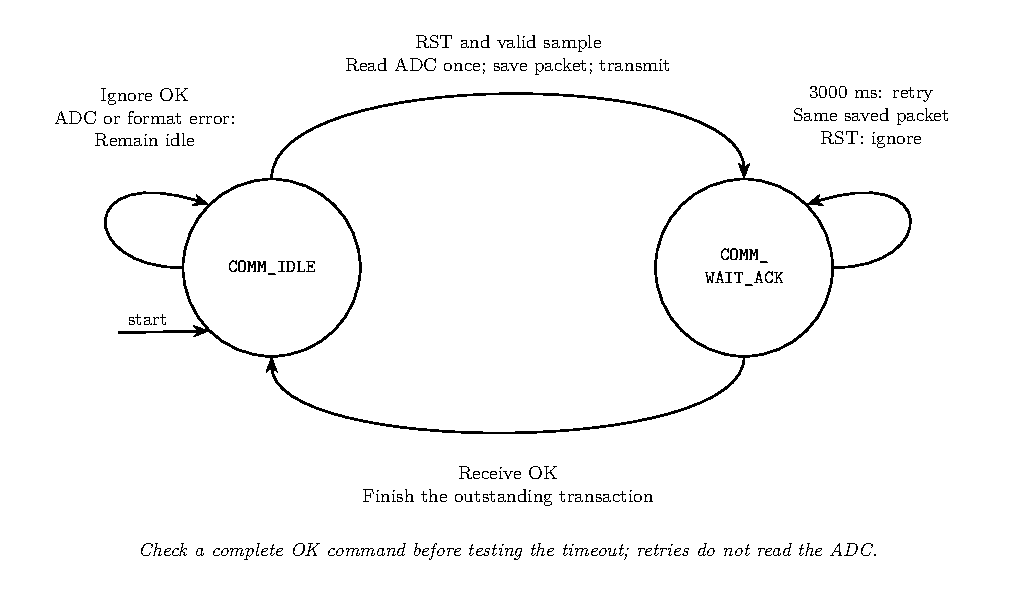
\includegraphics[width=\textwidth]{lab5_communication_fsm.pdf}
\caption{Request, saved-packet retransmission, and acknowledgment transitions.}
\label{fig:communication}\end{figure}

The start of every controller call consumes any pending mailbox command and
clears the published flag. A command is therefore an event, not a permanent
mode. If the current state does not accept it, that event is ignored rather
than kept for a future state. OK received while idle cannot acknowledge a
measurement requested later. RST received during an active transaction cannot
replace the saved measurement.


\topic{Sampling once and constructing the saved response}

\par\noindent\begin{minipage}{\linewidth}
\begin{lstlisting}[caption={Communication FSM with checked acquisition and saved-packet retries},firstnumber=1]
void uart_communication_fsm(void)
{
    Command command = CMD_NONE;

    if (command_flag) {
        command = command_data;
        command_flag = 0;
        command_data = CMD_NONE;
    }

    switch (state) {
    case COMM_IDLE:

        if (command == CMD_RST) {
            uint32_t sample;

            if (Sensor_ReadOnce(&sample) != HAL_OK) {
                adc_read_errors++;
                break;
            }

            int n = snprintf(packet, sizeof(packet), "!ADC=%lu#\r\n",
                             (unsigned long)sample);

            if (n <= 0 || n >= (int)sizeof(packet)) {
                uart_tx_errors++;
                break;
            }
            packet_length = (uint16_t)n;
            state = COMM_WAIT_ACK;
            SendSavedPacket();
        }
        break;
\end{lstlisting}
\end{minipage}\par

\par\noindent\begin{minipage}{\linewidth}
\begin{lstlisting}[caption={Communication FSM with checked acquisition and saved-packet retries (continued)},firstnumber=34]
    case COMM_WAIT_ACK:

        if (command == CMD_OK) {
            state = COMM_IDLE;
        } else if ((uint32_t)(HAL_GetTick() - last_tx_ms) >= 3000u) {

            SendSavedPacket();
        }

        break;

    default:
        state = COMM_IDLE;
        break;
    }
}
\end{lstlisting}
\end{minipage}\par

The response buffer has 20 positions. A bounded \code{snprintf} call constructs
the ADC frame and appends CR/LF.
The cast to unsigned long agrees with the \texttt{\%lu} conversion specifier.
The decimal digits represent the raw ADC count, not a voltage in volts.
For the sample 2048, the logical protocol frame is \texttt{!ADC=2048\#}.
The extra carriage return and line feed make the next terminal output appear
on a new line; they are display separators outside the protocol delimiters.

The formatting function returns the required character count excluding the
null terminator. A nonpositive result or a result at least as large as the
buffer capacity is rejected. Only a valid fitting string supplies
\code{packet_length}. Transmission uses that length, so the terminating zero
is not sent as part of the UART frame.

The largest 12-bit count contains four decimal digits. The corresponding
response occupies \(1+3+1+4+1+2=12\) transmitted characters: start delimiter,
ADC, equals sign, digits, end delimiter, and CR/LF. Including the C terminator
requires 13 buffer positions, so the 20-position array is sufficient. At 9600
baud, this twelve-character packet requires approximately
\[
T_{\mathrm{packet}}=12\times\frac{10}{9600}=12.5\ \mathrm{ms}.
\]


\topic{Three-second timeout and retransmission of identical data}

\par\noindent\begin{minipage}{\linewidth}
\begin{lstlisting}[caption={Transmit the saved packet and record the new waiting origin},firstnumber=1]
static void SendSavedPacket(void)
{
    if (HAL_UART_Transmit(&huart2, (uint8_t *)packet,
                          packet_length, 100) != HAL_OK) {
        uart_tx_errors++;
    }

    last_tx_ms = HAL_GetTick();
}
\end{lstlisting}
\end{minipage}\par

The timeout test computes the unsigned millisecond difference between
\code{HAL_GetTick()} and \code{last_tx_ms}, then compares it with 3000.
The timestamp is recorded after the transmit attempt returns. Thus, the waiting
interval begins at the end of that call, including when the call reports a
transmit error. The next retry is attempted on the first foreground visit at
or after the 3000-ms threshold. For a normal twelve-character response, the
interval between transmission starts is approximately 3000 ms plus 12.5 ms
of serial time and foreground overhead, rather than an exact three-second
start-to-start period.

The subtraction is performed with unsigned arithmetic. For example, if the
saved tick is \(2^{32}-1000\) and the current tick after rollover is 2000,
the unsigned difference is 3000. This permits the ordinary three-second
comparison to work across the millisecond-counter wrap, provided the check
is serviced within the intended elapsed-time range. There is no need to reset
the global tick or compare an absolute future deadline.

On timeout, \code{SendSavedPacket} transmits the existing byte string. It never
calls \code{Sensor_ReadOnce}. If the potentiometer is moved after the first
response but before acknowledgment, retries must still contain the previous
count. A new measurement becomes eligible only after OK returns the FSM to
idle and a later RST begins a new transaction. This preserves the meaning of
retransmission: repeat the same outstanding data, rather than silently change it.


\topic{Acknowledgment priority and protocol limits}

Inside the wait state, a completed OK command is checked before the timeout.
If both conditions are present when the controller is called, acknowledgment
wins and no retry occurs during that call. This priority concerns a fully
parsed command. If only part of an OK frame has arrived when the timeout is
checked, the current implementation can still resend before parsing finishes.

No retry limit is configured. Without OK, the controller keeps retrying the
same saved packet. A late or duplicated OK is not tagged with a transaction
number. Delimiters and exact command matching reject many malformed strings,
but they do not provide an end-to-end integrity check for a response value.
These characteristics define the scope of this small laboratory protocol and
explain why a production protocol may add sequence numbers, checksums, and
explicit retry limits.


\section{Main-loop integration and practical timing}

\topic{Initialization order and foreground service}

\par\noindent\begin{minipage}{\linewidth}
\begin{lstlisting}[caption={Application startup after peripheral initialization},firstnumber=1]
if (Sensor_Init(LAB5_PROTEUS_SIMULATION) != HAL_OK)
{
    Error_Handler();
}
UART_RxInit();
CommandParser_Init();
UART_Communication_Init();
uint32_t last_led_ms = HAL_GetTick();
\end{lstlisting}
\end{minipage}\par

\par\noindent\begin{minipage}{\linewidth}
\begin{lstlisting}[caption={Main-loop services and the independent LED heartbeat},firstnumber=1]
while (1)
{
    UART_RxService();
    command_parser_fsm();
    uart_communication_fsm();

    uint32_t now = HAL_GetTick();
    if ((uint32_t)(now - last_led_ms) >= 500u)
    {
        last_led_ms = now;
        HAL_GPIO_TogglePin(LED_RED_GPIO_Port, LED_RED_Pin);
    }
}
\end{lstlisting}
\end{minipage}\par

Peripheral initialization precedes application initialization. Sensor setup
must succeed before the application begins handling requests. Receive
initialization clears its queue and arms the first interrupt transfer; parser
initialization clears the token and mailbox; communication initialization
clears the packet length, state, timestamps, and diagnostic counters.

Each main-loop pass first offers UART recovery, then advances parsing by one
byte, then processes commands and timeout conditions. This order allows a
command completed by the parser to be consumed immediately during the same
pass. The LED check follows these services and does not call \code{HAL_Delay}.
Saving \code{last_led_ms = now} schedules its next toggle relative to actual
service time, so a long foreground delay can shift the blink phase. It does
not queue multiple missed LED transitions.


\topic{Receive capacity while foreground work is blocked}

At 9600 baud with ten bits per character, the maximum continuous arrival
rate is approximately 960 bytes/s. An initially empty 29-byte queue would
fill in approximately
\[
T_{\mathrm{fill}}=\frac{29}{960}\approx30.2\ \mathrm{ms}
\]
if the foreground removed no bytes. A normal twelve-character response occupies
about 12.5 ms of polling transmission. During that interval, UART receive
interrupts can continue, but the foreground parser cannot consume its queue.
About twelve incoming characters could accumulate at a continuous full-rate
input. This is compatible with the available capacity if the queue was
sufficiently empty, but it is not a guarantee for every burst pattern.

The transmit timeout is 100 ms. A stalled transmit attempt can therefore
block foreground service much longer than the queue's full-rate fill time.
ADC polling can also wait up to 10 ms on failure. Overflow detection and
frame invalidation are consequently meaningful even in a human-operated
terminal application. Bounded buffering absorbs short bursts; it does not
replace flow control for an indefinitely faster producer.

Parsing is bounded because each call handles at most one byte and token
comparison is limited to the small fixed strings. The acknowledgment wait
itself is nonblocking: no foreground loop waits in place for three seconds.
The distinction between nonblocking waiting and bounded blocking peripheral
calls explains both the responsiveness and the limits of this implementation.


\topic{Diagnostic information}

\begin{table}[htbp]\centering\small
\caption{Diagnostic variables and their purpose}
\begin{tabular}{p{55mm}p{91mm}}\toprule
Variable & Meaning\\\midrule
\code{uart_rx_dropped} & New bytes rejected because the receive queue was full.\\
\code{uart_rx_errors} & UART reception errors or failed receive rearming.\\
\code{adc_read_errors} & Accepted requests whose ADC acquisition failed.\\
\code{uart_tx_errors} & Packet formatting rejection or transmit failure.\\
\code{sensor_calibration_compat_used} & Indicates entry into the simulation compatibility branch; not itself an error counter.\\\bottomrule
\end{tabular}\end{table}

These variables can be inspected in the debugger. The protocol does not send
extra diagnostic messages, which keeps the terminal response format unchanged.
A transmit failure still updates the retry timestamp and waits before trying
again, avoiding a continuously executing failure loop. Receive faults take a
different recovery path: invalidate uncertain input and wait for a fresh frame.


\section{Simulation results and interpretation}

\topic{Midscale request and response}

Figure~\ref{fig:results} shows the running circuit with the potentiometer
around its midpoint. The voltmeter reads approximately 1.65 V and the terminal
contains repeated \texttt{!ADC=2048\#} responses. This agrees with the 12-bit
midscale calculation. The screenshot also contains RST and OK command text,
followed by another request and response. The LED is lit in this captured
instant, which is consistent with an active-high heartbeat output; a single
still image cannot measure its 500-ms toggle interval.

\begin{figure}[htbp]\centering
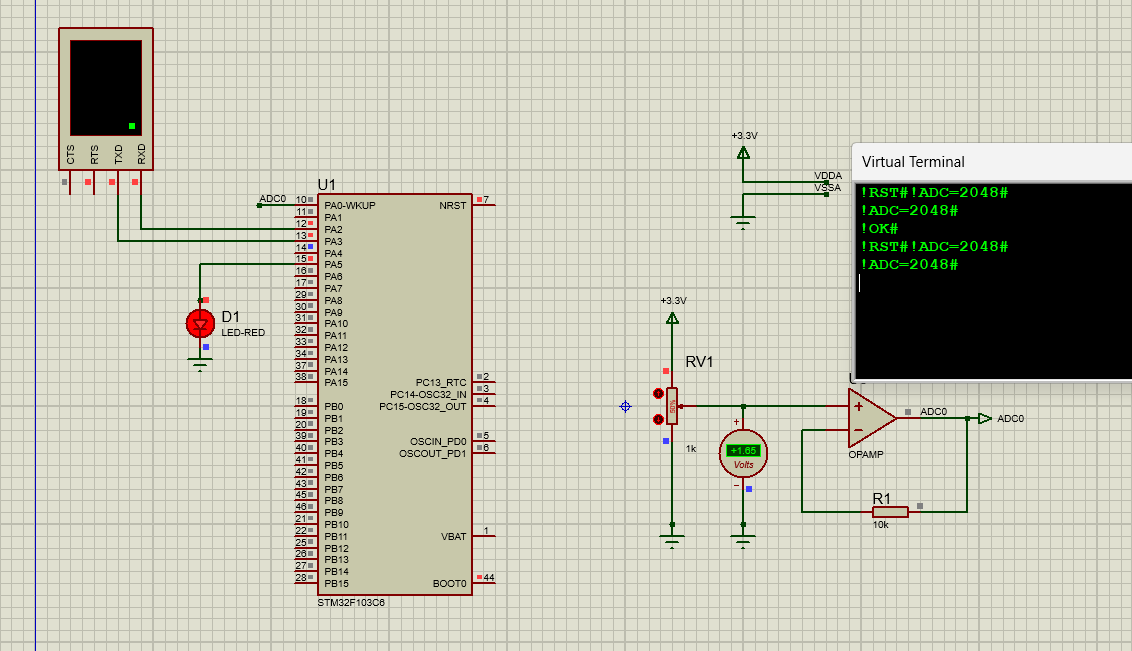
\includegraphics[width=\textwidth]{lab5_uart_results.png}
\caption{Simulation at approximately 1.65 V with ADC response frames containing 2048.}
\label{fig:results}\end{figure}

The first displayed request and response are adjacent on one line. This is
consistent with a locally echoed command ending in \texttt{\#} without a newline,
followed by the device response. The outgoing response then supplies CR/LF.
The final receive callback does not perform byte-by-byte echo, so visible
command characters should not be treated as proof of firmware loop-back.


\topic{Reading the visible transaction sequence}

The terminal first shows a request and an ADC response containing 2048,
then another ADC frame with the same value. Next, an OK command appears,
followed later in the visible sequence by another RST and two more 2048
responses. The repeated value agrees with the saved-packet behavior, while
the second request is consistent with starting another transaction after an
acknowledgment. Since the input remains around the same midpoint, a new
measurement can also legitimately equal the previous one.

The screenshot contains no time labels. It therefore cannot establish that
the repeated responses were exactly three seconds apart, how long output
remained silent after OK, or whether the input was changed between retries.
The three-second condition and preserved packet are explicit in the code;
the visible evidence establishes the frame format and midscale numerical
relationship. Separating these observations makes the result understandable
without attributing unrecorded timing measurements to a still image.


\topic{Additional observations that would complete verification}

A timed transaction trace would make timeout behavior explicit. Send RST
once, withhold OK, and record the first response plus at least two retries
with simulation-time labels. Then send OK and show an interval longer than
three seconds with no further response. This demonstrates both retry and
termination, rather than only showing the acknowledgment text.

To demonstrate that retransmission preserves the sample, request at one
potentiometer position, change the voltage before acknowledging, and observe
that retries retain the old count. After OK, send a new RST and show the count
changing to match the new voltage. Values near 0.825 V, 1.65 V, and 2.475 V
would ideally be near 1024, 2048, and 3072, respectively, with quantization
and reference assumptions as described earlier.

A separate loop-back capture would document the preliminary UART exercise.
CubeMX images of USART2 parameters, its enabled interrupt, and ADC channel 0
could supplement the configuration explanation; the numerical settings in
this text are already recoverable from the supplied initialization code.
The two supplied simulation images are included as actual results, while
these additional observations remain a verification procedure rather than
claimed completed experiments.


\section{Conclusion}

The completed design organizes UART communication into byte reception,
frame parsing, and transaction control. Interrupt-driven reception places
characters in a bounded ring buffer. The parser recognizes exact delimited
commands and publishes one command at a time. The communication FSM acquires
one checked ADC sample for a new request, stores its ASCII response, retries
that response after the acknowledgment timeout, and returns to idle on OK.

The 1.65-V simulation result and the reported count of 2048 agree with the
12-bit conversion model. The three-second wait is implemented using elapsed
HAL ticks, allowing foreground services and the heartbeat to continue between
transmissions. Packet preservation, length checking, receive-loss recovery,
and explicit ADC status handling explain how the implementation maintains a
coherent exchange even when input is incomplete or a peripheral operation
fails. These mechanisms provide a practical foundation for more capable
serial protocols with stronger integrity checks and transaction identification.


\clearpage
\phantomsection
\addcontentsline{toc}{section}{References}
\begin{thebibliography}{6}
\bibitem{lab}
Le Trong Nhan, \emph{Flow and Error Control in Communication},
Microcontroller Laboratory 5: UART, course handout, Ho Chi Minh City
University of Technology. Supplied laboratory document.
\bibitem{stm32}
STMicroelectronics, \emph{STM32F103x8 / STM32F103xB},
Datasheet DS5319, Rev.~20, July 2025. Available from the
\href{https://www.st.com/resource/en/datasheet/stm32f103c8.pdf}
{STMicroelectronics document archive}. Accessed: November 27, 2026.
\bibitem{hal}
STMicroelectronics, \emph{Description of STM32F1 HAL and Low-Layer Drivers},
User Manual UM1850. Peripheral API behavior was also checked against the
STM32F1 HAL driver sources included in the project. Available from the
\href{https://www.st.com/resource/en/user_manual/um1850-description-of-stm32f1-hal-and-lowlayer-drivers-stmicroelectronics.pdf}
{STMicroelectronics document archive}.
\bibitem{keil}
Arm Keil, ``\mbox{$\mu$Vision} User's Guide.'' Available from the
\href{https://www.keil.com/support/man/docs/uv4/default.htm}
{Keil documentation website}. Accessed: November 27, 2026.
\bibitem{proteus}
Labcenter Electronics, ``Proteus Design Suite: PCB design and circuit
simulation software.'' Available from the
\href{https://www.labcenter.com/}{Labcenter Electronics website}.
Accessed: November 27, 2026.
\end{thebibliography}
\end{document}
